\documentclass[11pt]{airesearch}
\usepackage[T1]{fontenc}
\usepackage{lmodern} 

%%%%%%%%%%%%%%%%%%%%%%%%%%%%%%%%%%%%%%%%%%%%%%%%%%%%%%%%%%%%%%%%%%%%%%%%%%%%%%%
%%% PACKAGES 
%
% Layout %%%%%%%%%%%%%%%%%%%%%%%%%%%%%%%%%%%%%%%%%%%%%%%%%%%%%%%%%%%%%%%%%%%%%%
\usepackage{fullpage}
\usepackage{wrapfig}
\setlist[itemize]{leftmargin=*,topsep=1pt,itemsep=1pt}

% Graphics & Diagrams
\usepackage{tikz}
\usetikzlibrary{shapes.geometric, arrows.meta, positioning, fit, calc, shadows}

% Algorithm %%%%%%%%%%%%%%%%%%%%%%%%%%%%%%%%%%%%%%%%%%%%%%%%%%%%%%%%%%%%%%%%%%%
\usepackage{algorithm}
\usepackage{algpseudocode} 

% Custom Command for Project Page
\newcommand{\projectpage}[1]{%
  \begin{center}
    \small
    \vspace{-1.25ex}
    \texttt{Project Page}: \url{#1}
  \end{center}
}

%%%%%%%%%%%%%%%%%%%%%%%%%%%%%%%%%%%%%%%%%%%%%%%%%%%%%%%%%%%%%%%%%%%%%%%%%%%%%%%
%%% CODE LISTING STYLE (Apple / Xcode Aesthetic)
%
\definecolor{applepink}{RGB}{188, 51, 133}   % Keywords (def, class, return)
\definecolor{applered}{RGB}{196, 26, 22}     % Strings
\definecolor{applegreen}{RGB}{50, 109, 116}  % Comments
\definecolor{applebg}{RGB}{250, 250, 250}    % Very light gray/white background
\definecolor{applegray}{RGB}{120, 120, 120}  % Line numbers
\definecolor{appleborder}{RGB}{230, 230, 230}% Subtle border

\lstdefinestyle{xcode}{
    backgroundcolor=\color{applebg},
    commentstyle=\itshape\color{applegreen},
    keywordstyle=\bfseries\color{applepink},
    numberstyle=\tiny\sffamily\color{applegray},
    stringstyle=\color{applered},
    basicstyle=\ttfamily\color{black},
    breakatwhitespace=false,
    breaklines=true,
    captionpos=b,
    keepspaces=true,
    numbers=left,
    numbersep=10pt,
    showspaces=false,
    showstringspaces=false,
    showtabs=false,
    tabsize=4,
    frame=single,                % Box around code
    frameround=tttt,             % Rounded corners
    rulecolor=\color{appleborder},
    framesep=5pt,
    xleftmargin=15pt,            % Indentation for the box
    xrightmargin=5pt
}
\lstset{style=xcode}

%%%%%%%%%%%%%%%%%%%%%%%%%%%%%%%%%%%%%%%%%%%%%%%%%%%%%%%%%%%%%%%%%%%%%%%%%%%%%%%
%%% TITLE & AUTHOR
\title{\Huge \bfseries Monadic Context Engineering}
\author{
    \textbf{Yifan Zhang}$^{1}$~~~~\textbf{Mengdi Wang}$^{1}$ \\[1.5mm]
    $^1$Princeton University\\[0.5mm]
    \texttt{yifzhang@princeton.edu}
}
\date{\today}

\begin{document}

\maketitle

%%%%%%%%%%%%%%%%%%%%%%%%%%%%%%
%%% Abstract
\begin{abstract}
The proliferation of Large Language Models (LLMs) has catalyzed a shift towards autonomous agents capable of complex reasoning and tool use. However, current agent architectures are frequently constructed using imperative, ad hoc patterns. This results in brittle systems plagued by difficulties in state management, error handling, and concurrency. This paper introduces \textbf{Monadic Context Engineering (MCE)}, a novel architectural paradigm leveraging the algebraic structures of Functors, Applicative Functors, and Monads to provide a formal foundation for agent design. MCE treats agent workflows as computational contexts where cross-cutting concerns, such as state propagation, short-circuiting error handling, and asynchronous execution, are managed intrinsically by the algebraic properties of the abstraction. We demonstrate how Monads enable robust sequential composition, how Applicatives provide a principled structure for parallel execution, and crucially, how \textbf{Monad Transformers} allow for the systematic composition of these capabilities. This layered approach enables developers to construct complex, resilient, and efficient AI agents from simple, independently verifiable components. We further extend this framework to describe Meta-Agents, which leverage MCE for generative orchestration, dynamically creating and managing sub-agent workflows through metaprogramming.
\end{abstract}

\projectpage{https://github.com/yifanzhang-pro/monadic-context-engineering}

%%%%%%%%%%%%%%%%%%%%%%%%%%%%%%
%%% Introduction
\section{Introduction}
\label{sec:introduction}

The vanguard of artificial intelligence research increasingly focuses on building autonomous agents: systems that reason, plan, and act to accomplish goals by interacting with environments~\citep{yao2022react, shinn2023reflexion}. While the cognitive capabilities of underlying LLMs are critical, the architectural challenge of orchestrating the operational loop, typically a cycle of \textit{Thought}, \textit{Action}, and \textit{Observation}, presents a formidable barrier to creating robust and scalable systems.

Engineers building these agents confront a recurring set of fundamental challenges. Paramount among these is the maintenance of state integrity, requiring the reliable propagation of memory, beliefs, and history across a sequence of potentially fallible operations. Simultaneously, agents require error resilience to gracefully handle real-world failures, such as API timeouts or malformed model outputs, without obfuscating core logic with defensive boilerplate. Furthermore, developers need logical composability to construct complex behaviors from independent units of logic, facilitating the seamless assembly, reordering, and substitution of steps.

Beyond sequential logic, modern agents demand robust concurrency to orchestrate multiple simultaneous actions without descending into the complexities of manual thread management. Ideally, the architecture should also strictly manage computational effects, separating deterministic logic from non-deterministic interactions with the external world. Finally, as systems scale, we must address agent orchestration, managing specialized teams of agents that can be formed dynamically to address novel problems without introducing chaotic interactions.

Current mainstream approaches are typically imperative, addressing these issues with improvisational solutions. Consequently, developers face highly coupled codebases with convoluted control flow, rendering the resulting agents difficult to test, debug, and evolve. The lack of a principled structure for managing state, failure, and concurrency leads to inherently brittle systems.

This architectural deficit is becoming more apparent as the community moves towards standardized interaction patterns, such as the Model Context Protocol (MCP)~\citep{mcp2024}, which demand robust and predictable orchestration logic. 

We propose that a solution resides in a powerful hierarchy of abstractions from functional programming and category theory: the Functor, the Applicative Functor, and the Monad~\citep{moggi1991, wadler1992}. These are not merely design patterns but formal algebraic structures that provide a standardized method to compose computations within a \textit{context}. A \textbf{Functor} allows one to apply a pure function to a value inside a context (mapping). An \textbf{Applicative} extends this by enabling the application of a wrapped function to a wrapped value, a structure essential for executing independent computations concurrently. Finally, a \textbf{Monad} allows for the sequencing of dependent operations where the subsequent computation is determined by the result of the previous one (binding).

This progression, culminating in the Monad's \texttt{bind} operation, allows us to construct a railway for computation. Each logical step acts as a station, while \texttt{bind} lays the track, ensuring the computational process proceeds smoothly on the \textit{success track}. If any step fails, \texttt{bind} automatically shunts the entire computation to a \textit{failure track}, bypassing subsequent stations to proceed directly to the destination. This paper details the design, implementation, and application of \texttt{AgentMonad}, a structure embodying these principles to bring profound benefits to AI agent engineering.

%%%%%%%%%%%%%%%%%%%%%%%%%%%%%%
%%% Main Body: The AgentMonad Design
\section{From Functors to Monads: The AgentMonad Design}
\label{sec:design}

To apply Monadic Context Engineering to AI agents, we introduce a specialized structure: the \texttt{AgentMonad}. The \textit{context} it manages is a composite structure encapsulating all critical aspects of an agent's execution. We build our understanding by following the classic Functor-Applicative-Monad progression.

\subsection{The Anatomy of the \texttt{AgentMonad}: A Monad Transformer Stack}
The core architectural challenge in agent design is managing multiple, overlapping concerns simultaneously. A single-agent operation might need to interact with an external API, handle possible failures, and update the internal memory or world model of the agent. Attempting to manage these concerns with naive nesting, for example, a type like \texttt{Task<Either<State<...>>>}, is unworkable. It forces developers to manually unwrap each layer of the context, reintroducing the deeply nested, callback-style code that monads are intended to eliminate.

The principled solution is the \textbf{Monad Transformer}, a concept from functional programming that allows for the systematic composition of monadic capabilities~\cite{liang1995monad}. A monad transformer, \texttt{T}, is a type constructor that takes an existing monad \texttt{M} and produces a new, more powerful monad, \texttt{T(M)}, that combines the behaviors of both. Crucially, transformers provide a \textbf{lift} operation ($\texttt{lift} : \texttt{M A} \to \texttt{T M A}$) that allows any computation in an inner monad to be seamlessly used within the context of the combined outer monad. This enables the creation of a layered stack of capabilities that share a single, unified interface.

The \texttt{AgentMonad} utilizes this technique to create a stack designed specifically for agentic workflows (Figure \ref{fig:transformer_stack}). At the base lies the \textbf{\texttt{IO} or \texttt{Task} Monad}, which manages interactions with the external world. This separates the description of an action from its execution, making behavior observable. We then apply the \textbf{\texttt{EitherT} Transformer}, which introduces short circuiting error handling. This directly models the requirements of specifications like the Model Context Protocol (MCP)~\cite{mcp2024}, where tool results must explicitly indicate success or failure. Finally, we wrap the stack in the \textbf{\texttt{StateT} Transformer}. 

The resulting type, \texttt{StateT S (EitherT E IO)}, represents a computation that is simultaneously stateful, fallible, and capable of side effects. A single \texttt{bind} operation on this composite structure correctly threads the state, checks for errors, and sequences external actions. Mathematically, this implies the shape $\mathrm{S} \to \mathrm{IO}(\mathrm{Either}(\mathrm{E}, (\mathrm{A}, \mathrm{S})))$, unifying all contexts into a single return type.

This layered construction provides a robust and formal foundation for agent architecture. The resulting \texttt{AgentMonad}, with its type signature \texttt{StateT S (EitherT E IO) A}, directly maps its algebraic structure to the primary challenges of agent engineering. It ensures interactions are observable, error handling is robust, state management is functional, and workflows are composable.

\begin{figure}[ht!]
\centering
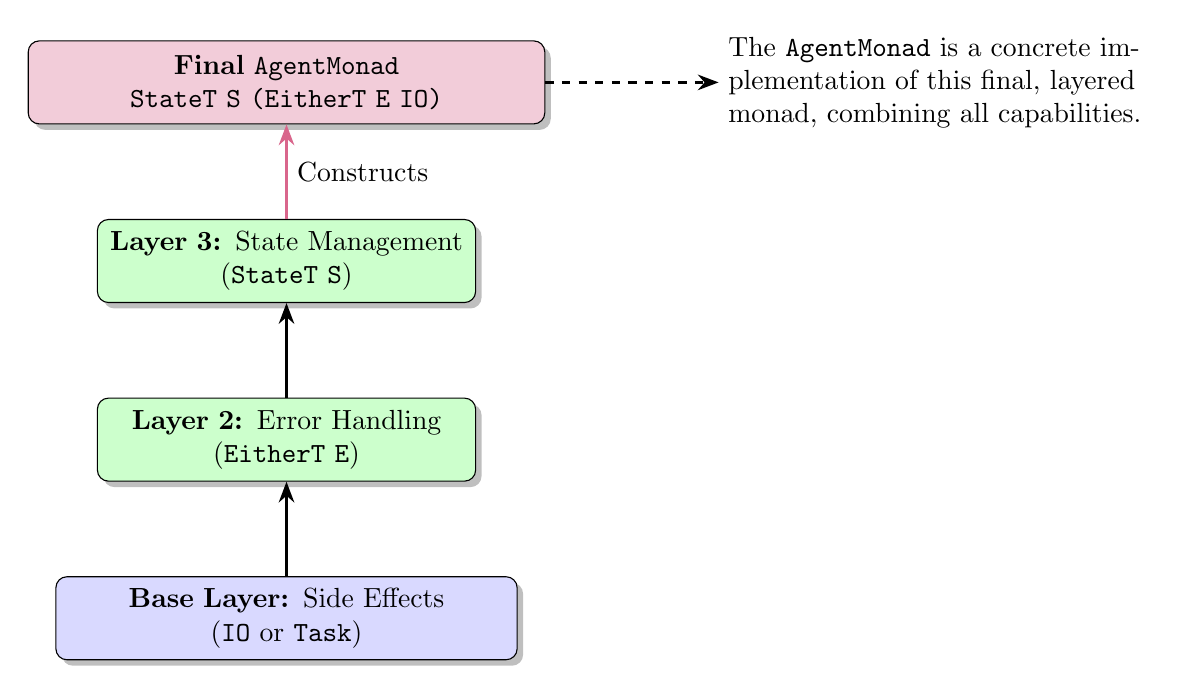
\begin{tikzpicture}[
    node distance=1.2cm, auto,
    monad/.style={rectangle, draw, fill=blue!15, text width=16em, text centered, rounded corners, minimum height=3em, drop shadow},
    transformer/.style={rectangle, draw, fill=green!20, text width=13em, text centered, rounded corners, minimum height=3em, drop shadow},
    arrow/.style={-Stealth, thick, rounded corners=5pt, line width=1pt}
]
    \node[monad] (base) {\textbf{Base Layer:} Side Effects \\ (\texttt{IO} or \texttt{Task})};
    \node[transformer, above=of base] (t1) {\textbf{Layer 2:} Error Handling \\ (\texttt{EitherT E})};
    \node[transformer, above=of t1] (t2) {\textbf{Layer 3:} State Management \\ (\texttt{StateT S})};
    \node[monad, above=of t2, fill=purple!20, text width=18em] (final) {\textbf{Final \texttt{AgentMonad}} \\ \texttt{StateT S (EitherT E IO)}};

    \draw[arrow] (base.north) -- (t1.south);
    \draw[arrow] (t1.north) -- (t2.south);
    \draw[arrow, purple!60] (t2.north) -- node[right, midway, text=black] {Constructs} (final.south);

    \node[right=of final, xshift=1cm, text width=15em] (desc) {The \texttt{AgentMonad} is a concrete implementation of this final, layered monad, combining all capabilities.};
    \draw[arrow, dashed] (final) -- (desc);

\end{tikzpicture}
\caption{Constructing the \texttt{AgentMonad} by stacking monad transformers. Each layer adds a new capability (context) to the monad below it, culminating in a single, unified structure that handles state, errors, and side effects.}
\label{fig:transformer_stack}
\end{figure}

\subsection{Level 1: AgentMonad as a Functor}
The most fundamental operation involves applying a pure function to the value inside our context without altering the context itself. This is the role of the Functor and its \texttt{map} operation.

The \textbf{map} function (or \texttt{fmap}) accepts a function $f: A \rightarrow B$ and an \texttt{AgentMonad[S, A]}, returning an \texttt{AgentMonad[S, B]}. It applies $f$ to the wrapped value while preserving the state and success status. Crucially, if the flow has already failed, \texttt{map} performs no operation.

\subsection{Level 2: AgentMonad as an Applicative Functor}
Applicatives extend Functors to handle a more complex scenario: what if the function we want to apply is \textit{also} wrapped in our context? This is particularly useful for combining the results of independent computations.

The \textbf{apply} operation (or \texttt{<*>}) takes an \texttt{AgentMonad} containing a function ($A \rightarrow B$) and an \texttt{AgentMonad} containing a value ($A$), returning a new context containing the result ($B$). This mechanism extracts the function and value from their respective contexts and applies them, ensuring state is propagated and failures are bypassed.

\subsection{Level 3: AgentMonad as a Monad}
The final and most powerful abstraction is the Monad. It addresses the core challenge of agent orchestration: sequencing operations where each step's logic depends on the result of the previous one.

The \textbf{bind} operation (often called \texttt{flatMap} or \texttt{then}) facilitates this chaining. It accepts an \texttt{AgentMonad[S, A]} and a function $f: A \rightarrow \text{AgentMonad}[S, B]$. The operation unwraps the value and state from the first context and passes them to $f$, which returns a new \texttt{AgentMonad}. This allows each step to alter the state or fail independently, with the state $S$ passed implicitly by the structure. The logic for \texttt{bind} is formalized in Algorithm~\ref{alg:bind} and visualized in Figure~\ref{fig:bind_logic}.

This structure abstracts away the repetitive and error prone boilerplate of state passing and error checking. The developer can focus entirely on defining the logic of each individual step.

\begin{figure}[ht!]
\centering
\resizebox{0.98\textwidth}{!}{
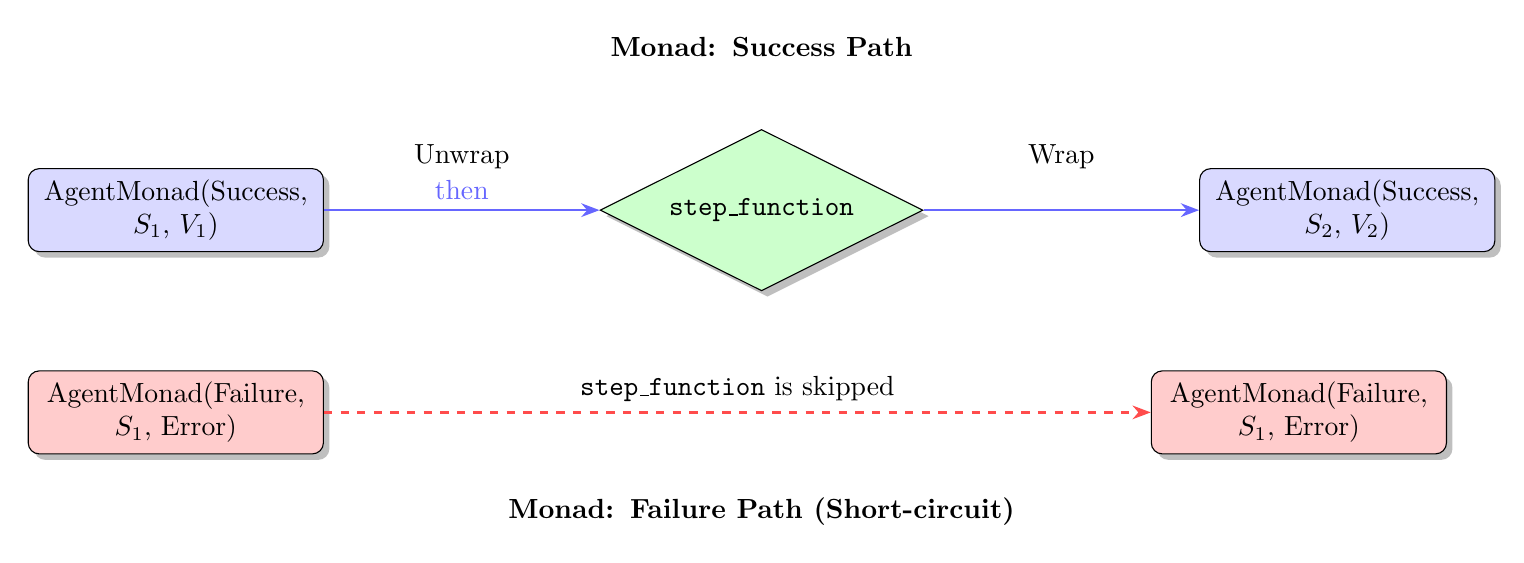
\begin{tikzpicture}[
    node distance=1.5cm and 3.5cm,
    auto,
    block/.style={rectangle, draw, fill=blue!15, text width=10em, text centered, rounded corners, minimum height=3em, drop shadow},
    fail_block/.style={rectangle, draw, fill=red!20, text width=10em, text centered, rounded corners, minimum height=3em, drop shadow},
    func_block/.style={diamond, draw, fill=green!20, text width=8em, text centered, minimum height=2em, aspect=2, drop shadow},
    arrow/.style={-Stealth, thick, rounded corners=5pt}
]
    % Success Path
    \node[block] (start_success) {AgentMonad(Success, $S_1$, $V_1$)};
    \node[func_block, right=of start_success] (func) {\texttt{\texttt{step\_function}}};
    \node[block, right=of func] (end_success) {AgentMonad(Success, $S_2$, $V_2$)};

    \draw[arrow, blue!60] (start_success) -- node[above] {then} (func);
    \draw[arrow, blue!60] (func) -- (end_success);
    \path (start_success.east) -- (func.west) node [midway, above, yshift=4mm] (text1) {Unwrap};
    \path (func.east) -- (end_success.west) node [midway, above, yshift=4mm] (text2) {Wrap};
    \node[above=0.8cm of func, text width=12em, align=center, font=\bfseries] {Monad: Success Path};

    % Failure Path
    \node[fail_block, below=of start_success] (start_fail) {AgentMonad(Failure, $S_1$, Error)};
    \node[fail_block, right=of start_fail, xshift=7cm] (end_fail) {AgentMonad(Failure, $S_1$, Error)};

    \draw[arrow, red!70, dashed] (start_fail.east) -- node[midway, above, text=black] {\texttt{\texttt{step\_function}} is skipped} (end_fail.west);
    \node[below=2.5cm of func, text width=20em, align=center, font=\bfseries] {Monad: Failure Path (Short-circuit)};

\end{tikzpicture}
}
\caption{Visualization of the Monad's \texttt{bind} operation. In the success path, the function is executed, transforming the entire context. In the failure path, the function is skipped, and the failure is propagated.}
\label{fig:bind_logic}
\end{figure}

\begin{algorithm}[H]
\caption{The \texttt{bind} (then) Operation Logic for AgentMonad}
\label{alg:bind}
\begin{algorithmic}[1]
\Procedure{then}{$\texttt{current\_flow}, \texttt{step\_function}$}
    \State \Comment{$\texttt{current\_flow}$ is an AgentMonad of $(status, state, value)$}
    \State \Comment{$\texttt{step\_function}$ is a function: $(state, value) \rightarrow \text{AgentMonad}'$}

    \If{$\texttt{current\_flow}.status$ is \textbf{FAILURE}}
        \State \Return $\texttt{current\_flow}$ \Comment{Short-circuit: propagate the failure without execution.}
    \EndIf

    \State \Comment{If successful, unwrap the container to get the current state and value.}
    \State $s \gets \texttt{current\_flow}.state$
    \State $v \gets \texttt{current\_flow}.value$

    \State \Comment{Execute the next step with the unwrapped values.}
    \State \textbf{try}
        \State $\texttt{next\_flow} \gets \texttt{step\_function}(s, v)$
    \State \textbf{catch} Exception $e$
        \State $\texttt{next\_flow} \gets \text{AgentMonad}(\textbf{FAILURE}, s, e)$ \Comment{Capture runtime exceptions as failures.}
    \State \textbf{end try}

    \State \Return $\texttt{next\_flow}$
\EndProcedure
\end{algorithmic}
\end{algorithm}

\section{Case Study: A Simple Research Agent}
\label{sec:case_study}
To demonstrate MCE in practice, we present a simple agent that answers the question: \textit{What is a Monad?}. We model the interaction of the agent with its tools using the structure of the Model Context Protocol (MCP)~\citep{mcp2024}, where the agent must process formal tool requests.

The agent logic is decomposed into four composable steps. First, \texttt{plan\_action} uses an LLM to formulate a plan which resolves into a structured MCP tool call. Second, \texttt{execute\_tool} consumes the request; if the tool exists, it is executed, and the monadic return value determines the structure of the resulting tool result block. Third, \texttt{synthesize\_answer} generates a final answer from the tool output. Finally, \texttt{format\_output} formats the final answer. Using \texttt{AgentMonad}, we chain these steps into a single, declarative workflow.

\begin{lstlisting}[caption={Chaining agent steps using Monadic Context Engineering.}, label=lst:chain, language=Python]
task = "What is a Monad?"
initial_state = AgentState(task=task)

# The agent logic is defined as a single, declarative, and robust chain.
final_flow = (
    AgentMonad.start(initial_state)
    .then(lambda s, _: plan_action(s, task))
    .then(lambda s, call: execute_tool(s, call))
    .then(synthesize_answer)
    .then(format_output)
)
\end{lstlisting}

\subsection{Robust Failure Handling}
The utility of MCE is most apparent during failure states, clarifying its synergy with protocols like MCP. Consider a scenario where the \texttt{plan\_action} step generates a request for a non-existent tool, such as `guess'.

In this sequence, the \texttt{plan\_action} step succeeds, returning an \texttt{AgentMonad} in a \texttt{Success} state. The monadic chain then passes this object to \texttt{execute\_tool}. The internal logic of the function attempts to dispatch the tool call, finds no tool named `guess', and returns an \texttt{AgentMonad} in a \texttt{Failure} state. This failure corresponds directly to creating an MCP tool result with an error flag.

Crucially, when the subsequent \texttt{.then(synthesize\_answer)} is called, the \texttt{bind} logic immediately detects the failure status and bypasses the rest of the chain. The \texttt{synthesize\_answer} function is never executed. The failure is propagated to the end of the chain, preserving the error message and the state at the point of failure. The final flow object cleanly reports failure without a single top-level conditional or exception block in the main orchestration logic, demonstrating the inherent resilience of the framework.

\section{Extending MCE for Concurrent and Parallel Orchestration}
\label{sec:async}

Modern AI agents often interact with multiple external services, such as querying several APIs for data or running different tools to gather diverse information. A purely sequential monadic chain, while robust, creates a performance bottleneck. To address this, MCE must handle asynchronous computations to provide a principled structure for \textit{concurrency} that enables effective I/O \textit{parallelism}.

While our core \texttt{AgentMonad} design, built on the transformer stack, can accommodate any base monad, specializing it for asynchronous operations unlocks significant performance gains. By instantiating our stack with a base \texttt{Task} or \texttt{Future} monad, common in modern programming languages for managing non-blocking I/O, we derive the \texttt{AsyncAgentMonad}, a structure purpose-built for high-performance agent orchestration.

\subsection{\texttt{AsyncAgentMonad}: A Monad Transformer in Practice}
The \texttt{AsyncAgentMonad} is the concrete implementation of our transformer stack. It provides a single, unified interface for chaining operations that are asynchronous, stateful, and fallible. An \texttt{AsyncAgentMonad[S, V]} does not hold a value directly; instead, it holds a \textit{promise} to eventually produce an \texttt{AgentMonad[S, V]}. The \texttt{bind} (\texttt{then}) operation chains asynchronous functions, allowing developers to write non-blocking I/O code that looks clean and sequential.

\begin{lstlisting}[language=Python, caption={Chaining asynchronous steps with \texttt{AsyncAgentMonad}.}, label=lst:async_chain]
task = "What is a Monad?"
initial_state = AgentState(task=task)

# Each step is now an async function that returns an AgentMonad.
async_flow = (
    AsyncAgentMonad.start(initial_state)
    .then(lambda s, _: async_plan_action(s, task))
    .then(async_execute_tool)
    .then(async_synthesize_answer)
    .then(async_format_output)
)

# The result is itself a promise, which must be awaited to run the flow.
final_result_flow = await async_flow.run()
\end{lstlisting}

\subsection{Unlocking True Parallelism via the Applicative Interface}
The most significant advantage of this extension emerges from the \textbf{Applicative} interface. While the Monad's \texttt{then} operation is inherently sequential (where step $N+1$ depends on step $N$), the Applicative's power lies in combining computations that are \textit{independent} of one another.

When the monadic context involves asynchronicity (like our \texttt{AsyncAgentMonad}), this distinction becomes critical. An Applicative combinator, which we will call \texttt{gather}, can take a list of independent \texttt{AsyncAgentMonad} instances and execute their underlying asynchronous operations \textit{concurrently}. On platforms supporting concurrent I/O or distributed execution, these tasks are effectively parallelized. The \texttt{gather} operation initiates all tasks simultaneously and waits for completion. It then collects their results into a single list within a new \texttt{AsyncAgentMonad}, correctly propagating state and aborting the entire group if any one of the tasks fails.

For example, consider an agent tasked with creating a daily briefing. It needs to fetch information from several independent sources: a news API, a weather service, and a stock market tracker. These tasks do not depend on each other and can be run in parallel to minimize latency.

\begin{lstlisting}[language=Python, caption={Parallel data gathering using an Applicative \texttt{gather} operation.}, label=lst:async_gather_code]
async def create_daily_briefing(state: AgentState, user_query: str) -> AgentMonad:
    # 1. Define independent, asynchronous tasks
    news_task = AsyncAgentMonad.start(state, user_query).then(async_fetch_news)
    weather_task = AsyncAgentMonad.start(state, user_query).then(async_fetch_weather)
    stocks_task = AsyncAgentMonad.start(state, user_query).then(async_fetch_stocks)

    # 2. Execute concurrently via Applicative 'gather'
    # The result is an AsyncAgentMonad that will resolve to a list of results
    gathered_data_flow = AsyncAgentMonad.gather([news_task, weather_task, stocks_task])

    # 3. Synthesize the collected results
    synthesis_step = await gathered_data_flow.then(async_synthesize_briefing).run()

    return synthesis_step
\end{lstlisting}


\begin{figure}[H]
\centering
\resizebox{0.98\textwidth}{!}{
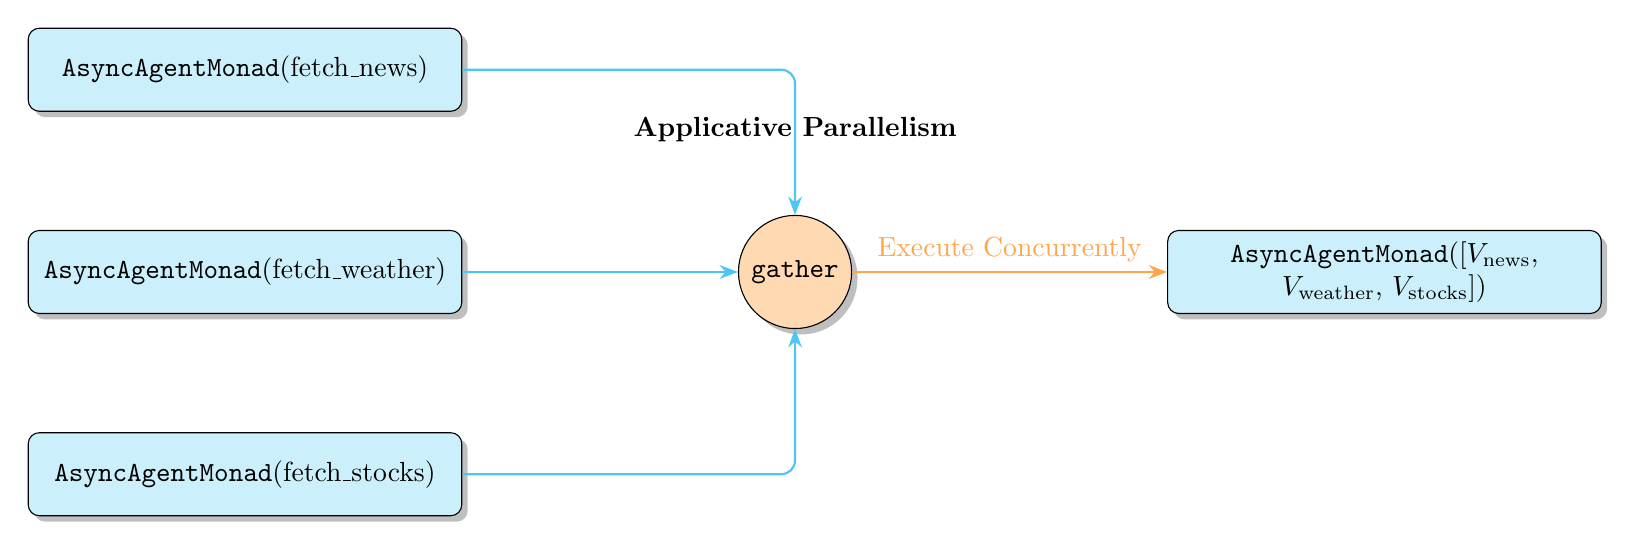
\begin{tikzpicture}[
    node distance=1.5cm and 2.0cm, auto,
    block/.style={rectangle, draw, fill=cyan!20, text width=15em, text centered, rounded corners, minimum height=3em, drop shadow},
    op/.style={circle, draw, fill=orange!30, minimum size=4em, drop shadow},
    arrow/.style={-Stealth, thick, rounded corners=5pt}
]
    \node[block] (task1) {\texttt{AsyncAgentMonad}(fetch\_news)};
    \node[block, below=of task1] (task2) {\texttt{AsyncAgentMonad}(fetch\_weather)};
    \node[block, below=of task2] (task3) {\texttt{AsyncAgentMonad}(fetch\_stocks)};
      
    \node[op, right=of task2, xshift=1.5cm] (gather) {\texttt{gather}};

    \node[block, right=of gather, text width=15em, xshift=2.0cm] (result) {\texttt{AsyncAgentMonad}([$V_{\mathrm{news}}$, $V_{\mathrm{weather}}$, $V_{\mathrm{stocks}}$])};

    \draw[arrow, cyan!70] (task1) -| (gather);
    \draw[arrow, cyan!70] (task2) -- (gather);
    \draw[arrow, cyan!70] (task3) -| (gather);
    \draw[arrow, orange!70] (gather) -- node[above] {Execute Concurrently} (result);

    \node[above=0.8cm of gather, text width=15em, align=center, font=\bfseries] {Applicative Parallelism};
\end{tikzpicture}
}
\caption{Parallel execution via an Applicative \texttt{gather} operation. Three independent asynchronous flows are initiated concurrently. The \texttt{gather} combinator waits for all to complete, then merges their results into a single flow. If any task fails, the entire gathered flow fails.}
\label{fig:async_gather}
\end{figure}

This pattern, visualized in Figure \ref{fig:async_gather}, is impossible to express elegantly with a purely monadic chain. A crucial consideration in this parallel model is the handling of state. Since each parallel flow could potentially modify the state, a merge strategy is required. A simple approach is to propagate the state from one predetermined flow, while more complex strategies could involve a custom merge function provided by the developer. Our framework defaults to the former for simplicity but acknowledges the need for more sophisticated state reconciliation in advanced use cases.

The combination of the Monad for sequencing dependent computations and the Applicative for executing independent computations in parallel provides a complete, robust, and high performance toolkit for orchestrating complex agent behaviors.

\section{MCE for Meta-Agents: Generative Orchestration}
\label{sec:meta_agent}
The robustness of an architectural pattern is demonstrated by its ability to scale in complexity and abstraction. We now elevate the MCE paradigm from orchestrating a single agent's workflow to orchestrating a \textit{team} of agents. We introduce a \textbf{Meta-Agent}: a higher-level agent whose primary function is not to solve the domain problem directly, but to dynamically create, configure, and supervise a team of specialized sub-agents. This approach is critical for tackling complex, multi-faceted problems that exceed the capabilities of a single monolithic agent.

\subsection{The Meta-Agent as a Metaprogrammer}
In this model, the Meta-Agent acts as a \textit{metaprogrammer}. Its operations do not manipulate domain data, but rather \textit{computational structures}, specifically, the monadic flows of its sub-agents. The `AgentMonad' of the Meta-Agent operates at a higher level of abstraction, where the state encompasses the entire system configuration, including active sub-agents and the overall plan. The values produced by steps in a Meta-Agent's flow are often fully formed `AgentMonad' workflows ready for execution.

The `bind' operation for a Meta-Agent becomes an act of generative orchestration. A step might take the overall goal, determine that a search capability is required, and output a new `AsyncAgentMonad' chain pre-configured for a search agent. This dynamically generated workflow is then executed, and its final result is fed back into the Meta-Agent's monadic context for the next step of supervision.

\subsection{Meta-Prompting for Dynamic Configuration}
A key mechanism for this dynamic configuration is meta-prompting~\citep{zhang2023meta, suzgun2024meta}. The Meta-Agent uses an LLM not to answer a question, but to generate the prompts and configurations for its sub-agents. For example, given a complex task, the Meta-Agent's first step might be a call to an LLM with a meta-prompt that requests a decomposition of the task into specialized roles. The result of this meta-prompt is then used by the Meta-Agent to programmatically construct and dispatch multiple sub-agents, each with a tailored monadic workflow (Figure \ref{fig:meta_agent}).

\begin{figure}[H]
\centering
\resizebox{\textwidth}{!}{
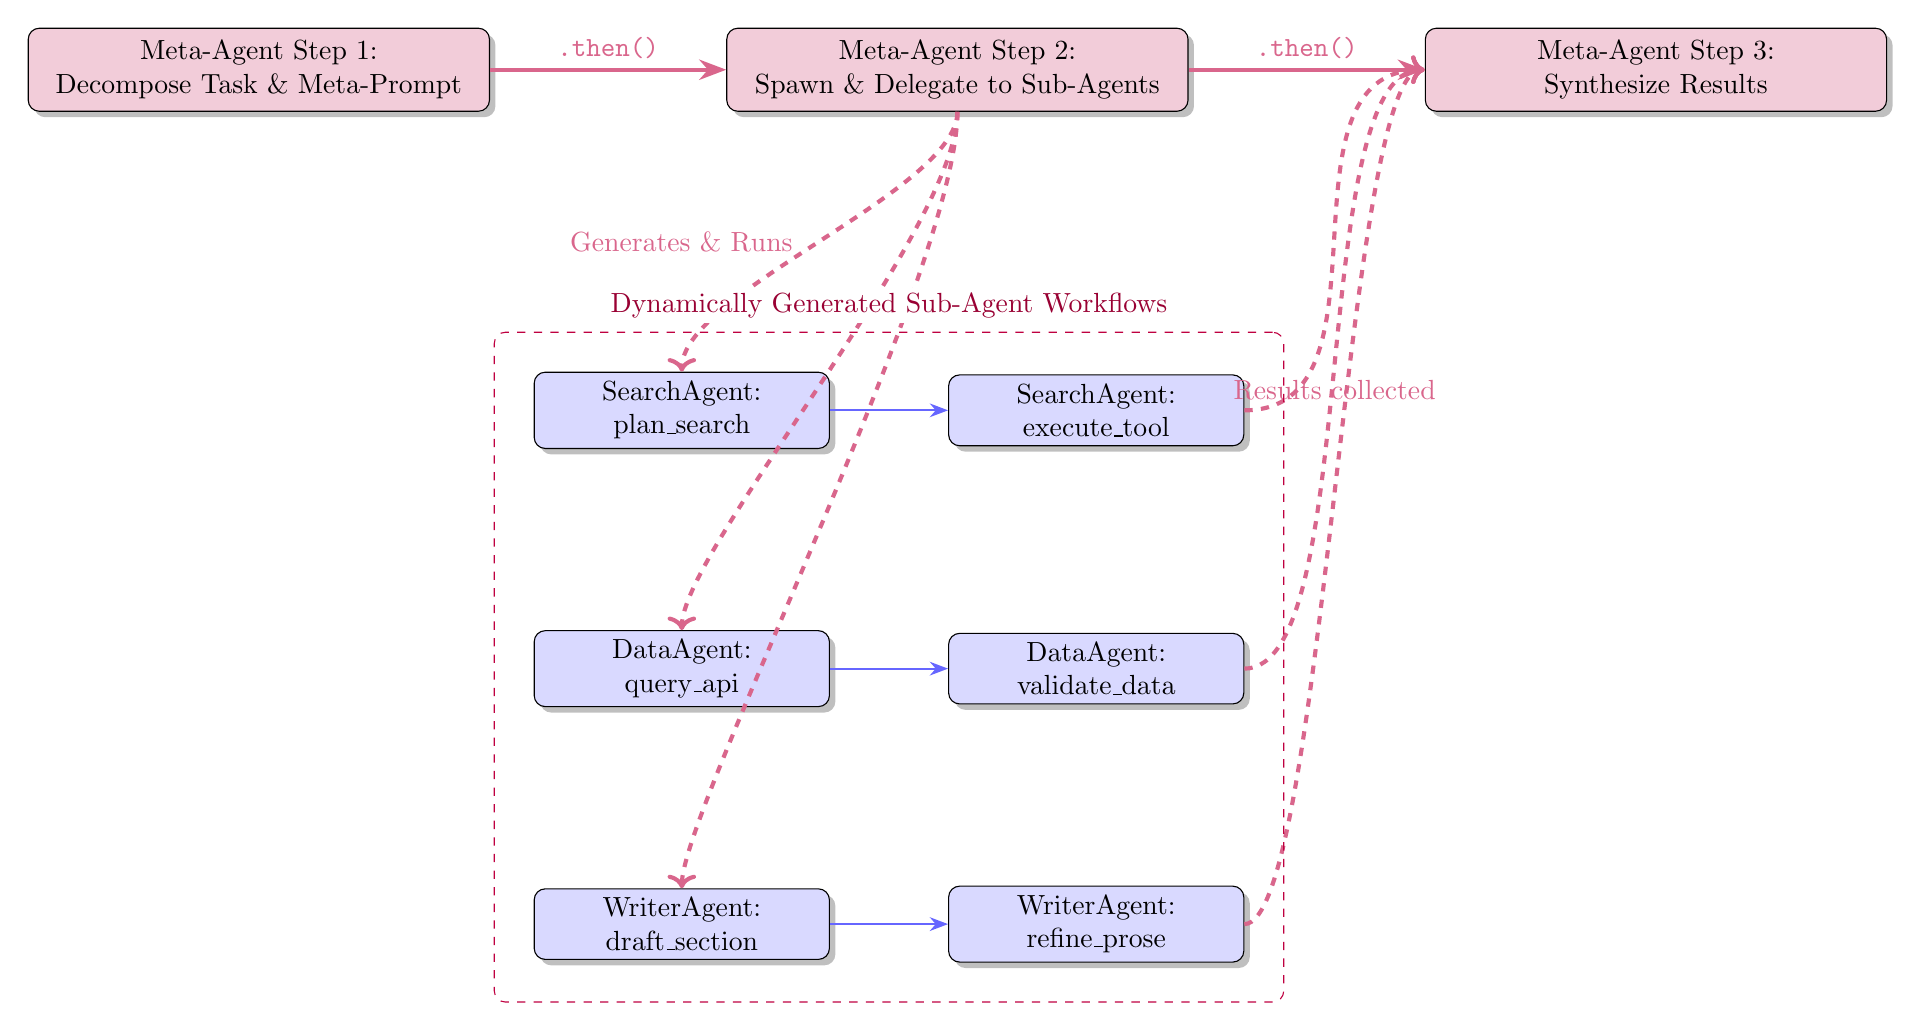
\begin{tikzpicture}[
    node distance=1.8cm and 1.5cm, auto,
    meta_block/.style={rectangle, draw, fill=purple!20, text width=16em, text centered, rounded corners, minimum height=3em, drop shadow},
    sub_block/.style={rectangle, draw, fill=blue!15, text width=10em, text centered, rounded corners, minimum height=2.5em, drop shadow},
    sub_flow/.style={-Stealth, thick, rounded corners=5pt, blue!60},
    meta_flow/.style={-Stealth, thick, rounded corners=5pt, purple!60, line width=1.5pt},
    mycontainer/.style={rectangle, draw=purple, dashed, rounded corners, inner sep=0.5cm}
]
    % Meta-Agent Flow
    \node[meta_block] (meta1) {Meta-Agent Step 1: \\ Decompose Task \& Meta-Prompt};
    \node[meta_block, right=of meta1, xshift=1.5cm] (meta2) {Meta-Agent Step 2: \\ Spawn \& Delegate to Sub-Agents};
    \node[meta_block, right=of meta2, xshift=1.5cm] (meta3) {Meta-Agent Step 3: \\ Synthesize Results};

    \draw[meta_flow] (meta1) -- node[above] {\texttt{.then()}} (meta2);
    \draw[meta_flow] (meta2) -- node[above] {\texttt{.then()}} (meta3);

    % Sub-Agent Flows
    \node[sub_block, below=of meta2, yshift=-1.5cm, xshift=-3.5cm] (subA1) {SearchAgent: \\ plan\_search};
    \node[sub_block, right=of subA1] (subA2) {SearchAgent: \\ execute\_tool};
    \draw[sub_flow] (subA1) -- (subA2);

    \node[sub_block, below=of subA1, yshift=-0.5cm] (subB1) {DataAgent: \\ query\_api};
    \node[sub_block, right=of subB1] (subB2) {DataAgent: \\ validate\_data};
    \draw[sub_flow] (subB1) -- (subB2);

    \node[sub_block, below=of subB1, yshift=-0.5cm] (subC1) {WriterAgent: \\ draft\_section};
    \node[sub_block, right=of subC1] (subC2) {WriterAgent: \\ refine\_prose};
    \draw[sub_flow] (subC1) -- (subC2);
      
    % Connections
    \draw[meta_flow, dashed, ->] (meta2.south) .. controls +(270:1) and +(90:1) .. (subA1.north) node[midway, left, xshift=-2mm] {Generates \& Runs};
    \draw[meta_flow, dashed, ->] (meta2.south) .. controls +(270:1.5) and +(90:1) .. (subB1.north);
    \draw[meta_flow, dashed, ->] (meta2.south) .. controls +(270:2) and +(90:1) .. (subC1.north);

    \draw[meta_flow, dashed, ->] (subA2.east) .. controls +(0:2) and +(180:2) .. (meta3.west);
    \draw[meta_flow, dashed, ->] (subB2.east) .. controls +(0:1.5) and +(180:1.5) .. (meta3.west) node[midway, below] {Results collected};
    \draw[meta_flow, dashed, ->] (subC2.east) .. controls +(0:1) and +(180:1) .. (meta3.west);

    % Container
    \node[mycontainer, fit=(subA1)(subC2)] (mycontainer) {};
    \node[above=0.1cm of mycontainer.north, fill=white, inner sep=2pt, text=purple!80!black] {Dynamically Generated Sub-Agent Workflows};

\end{tikzpicture}
}
\caption{A Meta-Agent's monadic flow. Each step of the Meta-Agent's \texttt{then} chain orchestrates the creation and execution of entire monadic workflows for specialized sub-agents. The results are then gathered back into the Meta-Agent's context for synthesis.}
\label{fig:meta_agent}
\end{figure}

\section{Related Work}
\label{sec:related_work}
The challenge of orchestrating agentic workflows is not new, and MCE builds upon a rich history of research in both AI and software engineering.

\noindent\textbf{Agent Frameworks}. Modern agent toolkits like LangChain~\citep{langchain} and LlamaIndex have introduced expression languages to chain components. Their \texttt{Runnable} protocol provides a degree of composability, often resembling a Functor or a limited Monad. However, state and error management are frequently handled as side channels rather than being intrinsic to the core abstraction. MCE offers a more formally grounded approach by unifying state, value, and error status into a single, cohesive monadic context, drawing from decades of established practice in functional programming for building robust systems~\citep{hudak2007history}.

\noindent\textbf{Multi-Agent Systems}. The paradigm of using multiple, collaborating agents to solve complex tasks has gained significant traction, exemplified by systems like AutoGen~\citep{autogen2023} and ChatDev~\citep{qian2023chatdev}. These frameworks typically rely on conversational managers or predefined topologies to orchestrate agent interactions. While powerful, their orchestration logic is often imperative and event-driven, which can make the overall system behavior difficult to predict and verify. MCE offers a complementary formal layer to these systems. A \textit{Meta-Agent} can use a monadic chain to formally define the process of agent creation, task delegation, and result synthesis, bringing the benefits of predictable state and error management to the multi-agent domain.

\noindent\textbf{Reasoning Paradigms}. High-level reasoning paradigms like ReAct~\citep{yao2022react}, Reflexion~\citep{shinn2023reflexion}, and the patterns in AutoGPT~\citep{autogpt} define the agent's cognitive cycle. MCE is not a replacement for these paradigms; rather, it is a superior low-level implementation framework. An entire ReAct loop can be modeled as a single \texttt{AgentMonad} step, which can then be composed with other steps with the guarantee that state and errors are managed robustly throughout.

\noindent\textbf{Model Context Protocol (MCP)}. Recently, there has been a push to standardize the communication layer between language models and external tools. A prominent example is the Model Context Protocol (MCP) introduced by Anthropic~\citep{mcp2024}. MCP proposes a standardized JSON-based format for models to request tool invocations and for the results to be returned to the model. The protocol explicitly includes fields like \texttt{tool\_id} for tracking requests and an \texttt{isError} flag in the result, formalizing the success or failure state of a tool call.
 
MCE and MCP are highly complementary and operate at different levels of abstraction. MCP standardizes the \textit{data interface}, the format of messages exchanged between the model and the agent's tool execution environment. In contrast, MCE provides a formal structure for the \textit{control flow} within the agent that processes these messages. For instance, an agent built with MCE would receive a \texttt{tools\_call} request, and the entire process of parsing the request, calling the corresponding tool, handling potential runtime exceptions, and packaging the output or error into an MCP-compliant \texttt{tool\_result} block can be encapsulated within a single, resilient monadic step. The \texttt{EitherT} layer of the \texttt{AgentMonad} directly maps to the \texttt{isError} flag in the MCP \texttt{tool\_result}, demonstrating a natural synergy between the two approaches. MCE provides the robust internal engine required to reliably implement the external contract defined by MCP. 

\noindent\textbf{Concurrent and Distributed Systems}. From a software engineering perspective, MCE is philosophically related to the Actor Model~\citep{hewitt1977actors}, which underpins systems like Erlang/OTP and Akka. Actors are independent agents that manage their own state and communicate via asynchronous messages. While the Actor Model excels at managing highly concurrent, distributed systems, MCE is specifically tailored for the goal-oriented, often sequential but parallelizable workflows of a single logical agent, providing a simpler and more direct abstraction for this common use case, with natural extensions towards parallelism via Applicatives.

\section{Conclusion}
\label{sec:conclusion}

Monadic Context Engineering provides a paradigm shift for AI agent development, advocating a transition from brittle imperative scripts to a principled, functional architecture. The benefits are immediate and significant. Agent logic becomes a clear, linear sequence of transformations where developers specify \textit{what} to do at each step, while the framework handles \textit{how} state, errors, and asynchronicity are propagated. The error model ensures that failures are handled gracefully and predictably, preventing corrupted states and unexpected crashes. Furthermore, agent behaviors are encapsulated in functions that can be independently tested and composed in novel ways to build increasingly complex agents. Finally, state is managed explicitly through the monadic flow, while the combination of Monad and Applicative interfaces provides a unified model for both sequential and concurrent execution, enabling parallelism.

In essence, MCE is the application of a mature, powerful idea from computer science to address the acute pain points of a new and rapidly evolving domain. By adopting these principled algebraic structures, the AI community can build more reliable, scalable, and understandable agents, laying a solid engineering foundation on the path toward more general and capable artificial intelligence.
 
\vspace{5ex}
\bibliographystyle{plainnat}
\bibliography{reference}

\clearpage
\appendix

\section{Conceptual Python Implementation}
\label{sec:appendix_impl}

Below are aligned excerpts of the \texttt{AgentMonad} and \texttt{AsyncAgentMonad} implementations, along with the reference step functions used in this paper.

\begin{lstlisting}[caption={Conceptual Implementation of the AgentMonad Class.}, label=lst:agentmonad, language=Python]
from __future__ import annotations

from collections.abc import Callable
from dataclasses import dataclass
from typing import Any, Generic, TypeVar, cast

from mce.models import AgentState, ToolCall, ToolRegistry, default_registry

S = TypeVar("S")
V = TypeVar("V")
R = TypeVar("R")


@dataclass(frozen=True)
class AgentMonad(Generic[S, V]):
    """Monadic container for stateful, fallible agent steps."""

    state: S
    value: V | None
    is_successful: bool = True
    error_info: Any = None

    def _require_value(self) -> V:
        if self.value is None:
            raise ValueError("AgentMonad has no value.")
        return self.value

    def then(self, func: Callable[[S, V], AgentMonad[S, R]]) -> AgentMonad[S, R]:
        if not self.is_successful:
            return AgentMonad.failure(self.state, self.error_info)
        try:
            value = self._require_value()
            return func(self.state, value)
        except Exception as exc:
            return AgentMonad.failure(self.state, exc)

    def map(self, func: Callable[[V], R]) -> AgentMonad[S, R]:
        if not self.is_successful:
            return AgentMonad.failure(self.state, self.error_info)
        value = self._require_value()
        return AgentMonad.success(self.state, func(value))

    def apply(self, func_flow: AgentMonad[S, Callable[[V], R]]) -> AgentMonad[S, R]:
        if not self.is_successful or not func_flow.is_successful:
            error = self.error_info if not self.is_successful else func_flow.error_info
            return AgentMonad.failure(self.state, error)
        func = func_flow._require_value()
        return self.map(func)

    @staticmethod
    def start(state: S, initial_value: V | None = None) -> AgentMonad[S, V]:
        value = initial_value if initial_value is not None else cast(V, state)
        return AgentMonad(state, value)

    @staticmethod
    def success(state: S, value: V) -> AgentMonad[S, V]:
        return AgentMonad(state, value, is_successful=True)

    @staticmethod
    def failure(state: S, error_info: Any) -> AgentMonad[S, V]:
        return cast(
            AgentMonad[S, V],
            AgentMonad(state, None, is_successful=False, error_info=error_info),
        )


# --- Example: Defining the agent's behavioral steps ---
def plan_action(state: AgentState, task: str) -> AgentMonad[AgentState, ToolCall]:
    call = ToolCall(tool_id="tool-1", name="search", arguments={"query": task})
    next_state = state.with_history(f"Plan: call {call.name} with query='{task}'.")
    return AgentMonad.success(next_state, call)


def execute_tool(
    state: AgentState, call: ToolCall, registry: ToolRegistry | None = None
) -> AgentMonad[AgentState, str]:
    registry = registry or default_registry()
    result = registry.run(state, call)
    next_state = state.with_history(f"Tool Result ({call.name}): {result.content}")
    if result.is_error:
        return AgentMonad.failure(next_state, result.content)
    return AgentMonad.success(next_state, result.content)


def synthesize_answer(state: AgentState, tool_output: str) -> AgentMonad[AgentState, str]:
    answer = (
        "Monadic Context Engineering structures agent workflows as composable steps "
        "with built-in state threading, error short-circuiting, and optional parallelism. "
        f"Evidence: {tool_output}"
    )
    next_state = state.with_history("Synthesized final answer.")
    return AgentMonad.success(next_state, answer)


def format_output(state: AgentState, answer: str) -> AgentMonad[AgentState, str]:
    formatted = f"Final Report:\n{answer}"
    next_state = state.with_history("Formatted response for delivery.")
    return AgentMonad.success(next_state, formatted)
\end{lstlisting}

\section{Conceptual AsyncAgentMonad Implementation}
\label{sec:appendix_async_agentmonad}

\begin{lstlisting}[caption={Conceptual Implementation of AsyncAgentMonad.}, label=lst:async_agentmonad, language=Python]
from __future__ import annotations

import asyncio
from collections.abc import Awaitable, Callable, Sequence
from typing import Any, Generic, TypeVar, cast

S = TypeVar("S")
V = TypeVar("V")
R = TypeVar("R")

AsyncStep = Callable[[S, V], Awaitable[AgentMonad[S, R]]]


class AsyncAgentMonad(Generic[S, V]):
    """Async monadic container for parallel, stateful, fallible workflows."""

    def __init__(self, run_func: Callable[[], Awaitable[AgentMonad[S, V]]]) -> None:
        self._run = run_func

    async def run(self) -> AgentMonad[S, V]:
        return await self._run()

    def then(self, func: AsyncStep[S, V, R]) -> AsyncAgentMonad[S, R]:
        async def new_run() -> AgentMonad[S, R]:
            current_flow = await self.run()
            if not current_flow.is_successful:
                return AgentMonad.failure(current_flow.state, current_flow.error_info)
            try:
                value = current_flow._require_value()
                return await func(current_flow.state, value)
            except Exception as exc:
                return AgentMonad.failure(current_flow.state, exc)

        return AsyncAgentMonad(new_run)

    @staticmethod
    def start(state: S, initial_value: V | None = None) -> AsyncAgentMonad[S, V]:
        async def run_func() -> AgentMonad[S, V]:
            return AgentMonad.start(state, initial_value)

        return AsyncAgentMonad(run_func)

    @staticmethod
    def gather(
        flows: Sequence[AsyncAgentMonad[S, Any]],
        merge_state: Callable[[Sequence[S]], S] | None = None,
    ) -> AsyncAgentMonad[S, list[Any]]:
        async def new_run() -> AgentMonad[S, list[Any]]:
            if not flows:
                return AgentMonad.failure(cast(S, None), "No flows provided")

            results = await asyncio.gather(*(flow.run() for flow in flows))
            errors = [result for result in results if not result.is_successful]
            if errors:
                failing = errors[0]
                return AgentMonad.failure(failing.state, failing.error_info)

            states = [result.state for result in results]
            final_state = merge_state(states) if merge_state else states[-1]
            values = [result.value for result in results]
            return AgentMonad.success(final_state, values)

        return AsyncAgentMonad(new_run)
\end{lstlisting}

\end{document}
